\documentclass[fleqn, xcolor=x11names]{beamer}
\usetheme{Frankfurt} % шаблон
\usecolortheme{default} % цветовая схема
\usepackage[11pt]{moresize}
\usepackage{multimedia}
\usepackage[T1]{fontenc}
\usepackage{pgfplots}
\usepackage[utf8]{inputenc}
\usepackage[russian]{babel}
\usepackage{media9}
\usepackage{listings}
\usepackage{amsmath}
\usepackage{color}
\usepackage{parskip}
\usepackage{wrapfig}

\usepackage{graphicx}
\lstdefinestyle{myLatexStyle}{
    basicstyle=\small\ttfamily,
    language={python},
    numbersep=5mm, numbers=left, numberstyle=\tiny, % number style
    breaklines=true,frame=single,framexleftmargin=8mm, xleftmargin=8mm,
    backgroundcolor=\color{green!5}, frameround=fttt,escapeinside=??,
    rulecolor=\color{red},
    morekeywords={% Give keywords here
        numpy},
    keywordstyle=\color[rgb]{0,0,1},                    % keywords
        commentstyle=\color[rgb]{0.133,0.545,0.133},    % comments
        stringstyle=\color[rgb]{0.627,0.126,0.941}  % strings
}
\lstset{style=myLatexStyle}

\setbeamertemplate{navigation symbols}{}
\setbeamertemplate{footline}{%
    \hspace{0.99\paperwidth}%
    \usebeamerfont{title in head/foot}%
    \insertframenumber\,/\,\inserttotalframenumber%
}



\title{GCNN}
\author[Медведев~Д.\,В.]{Медведев Алексей Владимирович}
\institute[ВМК МГУ]{МГУ имени М. В. Ломоносова,
факультет ВМК, кафедра ММП}
\date{} 

\begin{document}

\begin{frame}
\maketitle
\end{frame}

\begin{frame}[fragile]\frametitle{Зачем?}
\begin{block}{}
\begin{itemize}

\item Данные представлены в виде графа (например молекулы).

\item Можно обучать классификаторы для multilabeling.

\item Предсказание и распознавание действий.
\end{itemize}
\end{block}

\begin{figure}[h]
\begin{center}
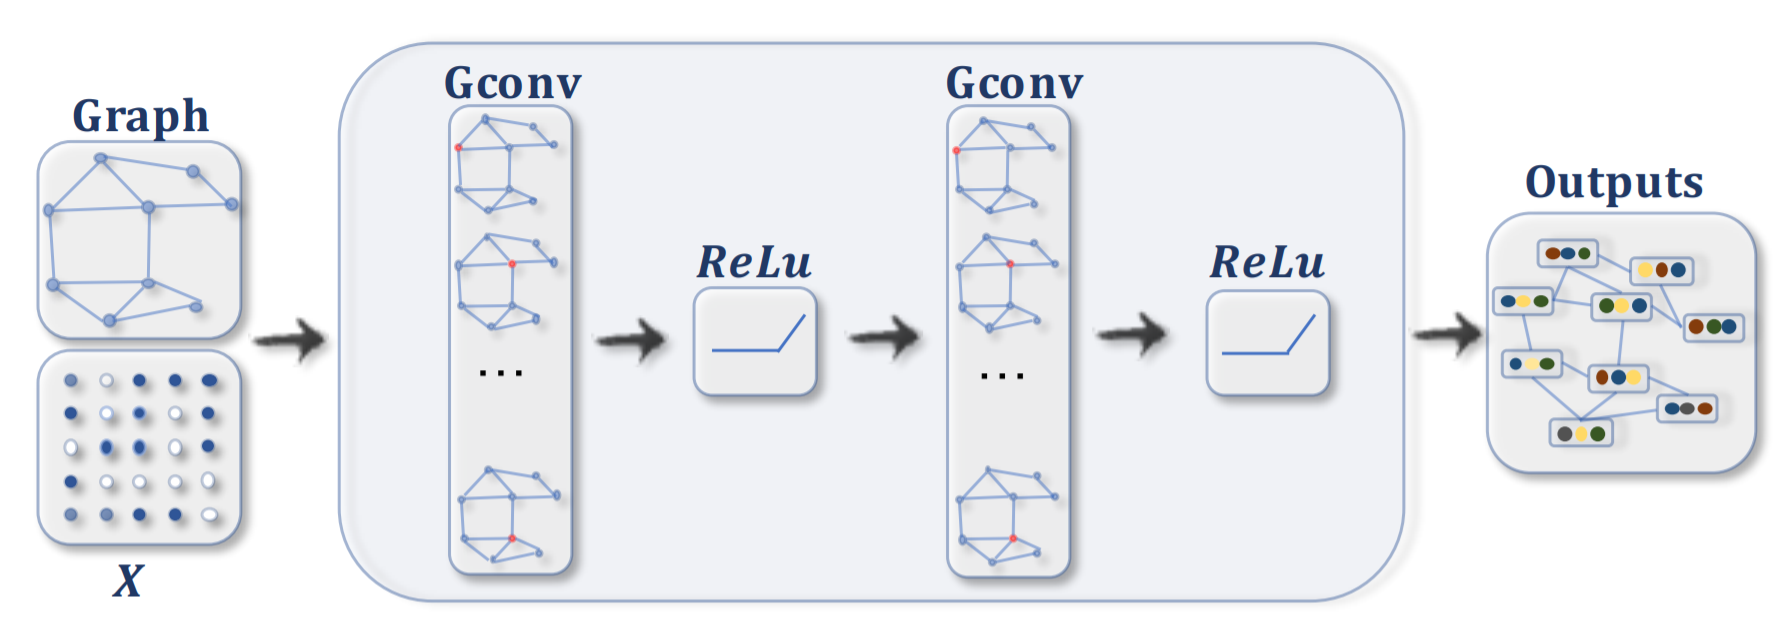
\includegraphics[scale=0.18]{/home/alex/python/Master_course/scientific_diary_2019-2020/slides/pics/GCNN-major.png}
\end{center}
\end{figure}

\end{frame}

\begin{frame}\frametitle{Спектральные сети}

$$L = D-A\;; L = I_N-D^{-0.5}AD^{-0.5}$$
$$\hat{f}(\lambda_l) = \sum \limits_{i=1}^{N} f(i)u_l(i)\;;f(i)= \sum \limits_{l=0}^{N-1} \hat{f}(\lambda_l)u_l(i)$$
$$\mathcal{F}(x)=U^Tx\;;\mathcal{F}^{-1}(x)=U\hat{x}$$

\end{frame}


\begin{frame}\frametitle{Спектральные сети}

\begin{figure}[h]
\begin{center}
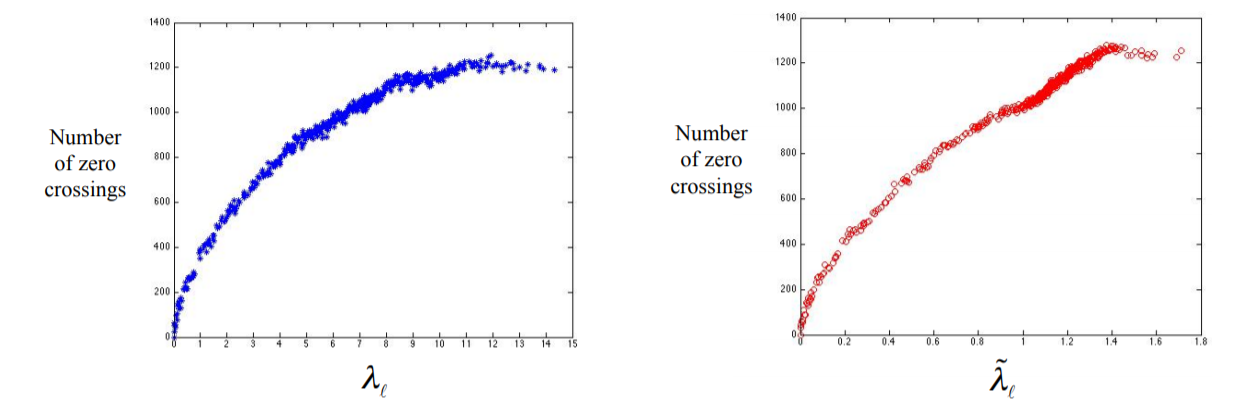
\includegraphics[scale=0.27]{/home/alex/python/Master_course/scientific_diary_2019-2020/slides/pics/laplacian_eigenvectors_property.png}
\end{center}
\end{figure}

$$ \mathcal{Z}_{\mathcal{G}}(f) := {e=(i,j)\in \mathcal{E}:f(i)f(j)<0} $$

\end{frame}

\begin{frame}\frametitle{Спектральные сети}

\begin{block}{Свертка}
$$ x *_{G} g = \mathcal{F}^{-1}(\mathcal{F}(x)\odot\mathcal{F}(g))=U(U^Tx\odot U^Tg) =$$
$$ \{g_{\theta}=diag(U^Tg)\}=Ug{_\theta}U^Tx$$
\end{block}

\end{frame}

\begin{frame}\frametitle{T. N. Kipf and M. Welling 2017 ICLR
}

\begin{block}{Чебышев}
$$ T_k(x) = 2 x T_{k-1}(x) - T_{k-2}(x)$$
$$T_0(x) = 1\;; T_1(x) = x$$
$$ x *_{G} g \approx \sum \limits_{k=0}^{K} \theta_k T_k(L)x $$
\end{block}

\begin{block}{GCN}
$$ x *_{G} g \approx \theta_0 x + \theta_1 (L-I_N)x=\theta_0 x-\theta_1 D^{-0.5}AD^{-0.5} x$$

$$ x *_{G} g \approx \theta(I_N + D^{0.5}AD^{-0.5})x $$
\end{block}

\end{frame}

\begin{frame}\frametitle{T. N. Kipf and M. Welling 2017 ICLR}

\begin{block}{Renormalization trick}
$$ I_N + D^{-0.5}AD^{-0.5} \rightarrow \tilde{D}^{-0.5}\tilde{A}\tilde{D}^{-0.5} $$
$$ \tilde{A} = A+I_N\; ; \tilde{D}_{ii} = \sum_j\tilde{A}_{ij}$$
$$ H^{(l+1)} = \sigma(	\tilde{D}^{-0.5}\tilde{A}\tilde{D}^{-0.5}H^{(l)}W^{(l)})$$
\end{block}

\end{frame}

\begin{frame}\frametitle{T. N. Kipf and M. Welling 2017 ICLR}

\begin{figure}[h]
\begin{center}
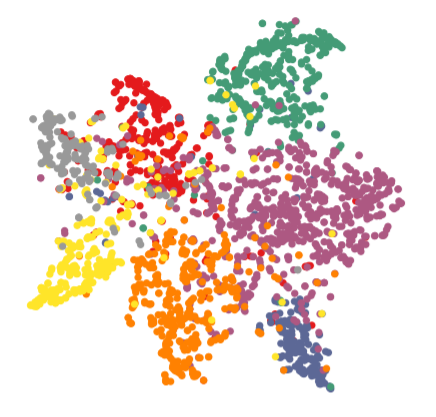
\includegraphics[scale=0.27]{/home/alex/python/Master_course/scientific_diary_2019-2020/slides/pics/Cora_tsne.png}
\caption{Cora dataset t-SNE}
\end{center}
\end{figure}

\end{frame}

\begin{frame}\frametitle{\footnotesize{Multi-Label Image Recognition with Graph Convolutional Networks\\
Zhao-Min Chen, Xiu-Shen Wei, Peng Wang, Yanwen Guo 2019 CVPR
}}

\begin{figure}[h]
\begin{center}
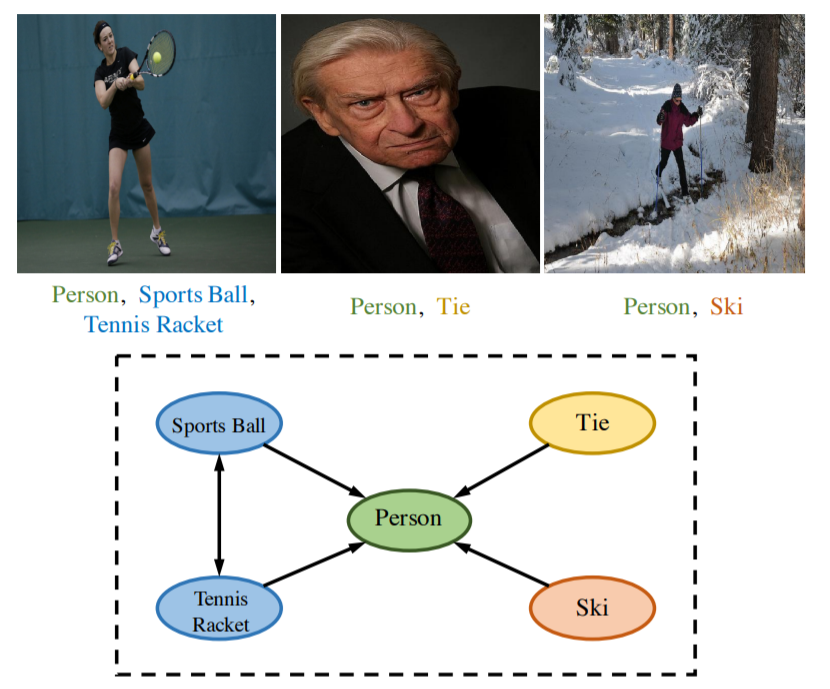
\includegraphics[scale=0.27]{/home/alex/python/Master_course/scientific_diary_2019-2020/slides/pics/Multilabel_problem.png}
\end{center}
\end{figure}

\end{frame}

\begin{frame}\frametitle{\footnotesize{Multi-Label Image Recognition with Graph Convolutional Networks\\
Zhao-Min Chen, Xiu-Shen Wei, Peng Wang, Yanwen Guo 2019 CVPR
}}

\begin{figure}[h]
\begin{center}
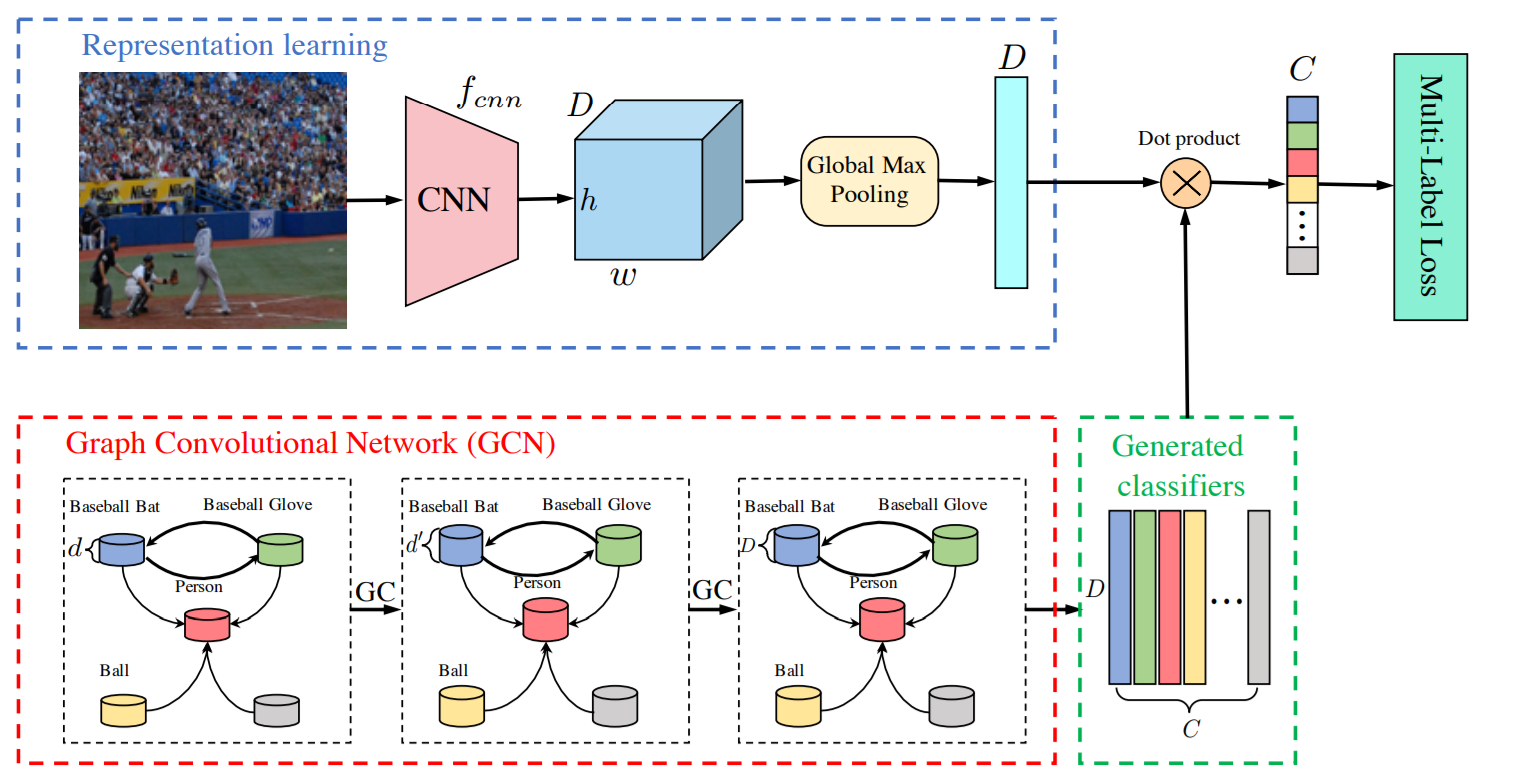
\includegraphics[scale=0.2]{/home/alex/python/Master_course/scientific_diary_2019-2020/slides/pics/Multilabel_svheme.png}
\end{center}
\end{figure}

\end{frame}

\begin{frame}\frametitle{\footnotesize{Multi-Label Image Recognition with Graph Convolutional Networks\\
Zhao-Min Chen, Xiu-Shen Wei, Peng Wang, Yanwen Guo 2019 CVPR
}}

\begin{block}{Adjacency matrix binary}
$$ P_i = M_i/N_i $$
$$ A_{ij} = \begin{cases}0, &\mbox{if } P_{ij} < \tau \\
1, & \mbox{else} \end{cases}$$
\end{block}

\begin{block}{Adjacency matrix reweighted}
$$ A_{ij} = \begin{cases}p/\sum \limits_{j=1,\;j\neq i}^C A_{ij} &\mbox{if } i\neq j\\
1-p, & \mbox{else} \end{cases}$$
\end{block}

\end{frame}

\begin{frame}\frametitle{\footnotesize{Multi-Label Image Recognition with Graph Convolutional Networks\\
Zhao-Min Chen, Xiu-Shen Wei, Peng Wang, Yanwen Guo 2019 CVPR
}}

\begin{figure}[h]
\begin{center}
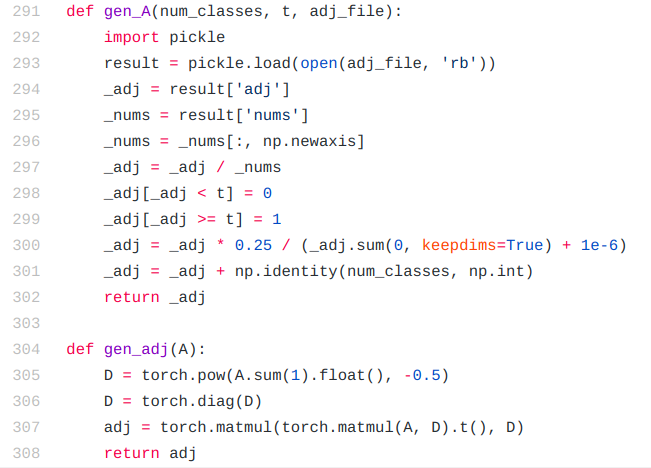
\includegraphics[scale=0.4]{/home/alex/python/Master_course/scientific_diary_2019-2020/slides/pics/Code_multilabel.png}
\end{center}
\end{figure}

\end{frame}

\begin{frame}\frametitle{\footnotesize{Multi-Label Image Recognition with Graph Convolutional Networks\\
Zhao-Min Chen, Xiu-Shen Wei, Peng Wang, Yanwen Guo 2019 CVPR
}}
\begin{figure}[h]
\begin{center}
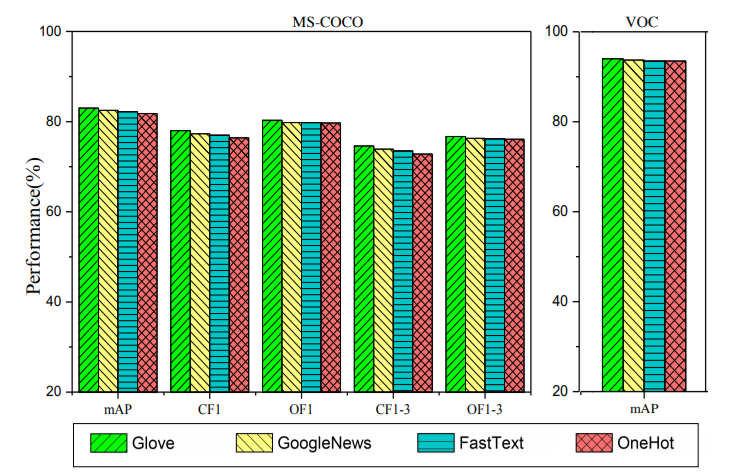
\includegraphics[scale=0.4]{/home/alex/python/Master_course/scientific_diary_2019-2020/slides/pics/Embeddings_Multilabel.png}
\end{center}
\end{figure}

\end{frame}

\begin{frame}\frametitle{\footnotesize{Multi-Label Image Recognition with Graph Convolutional Networks\\
Zhao-Min Chen, Xiu-Shen Wei, Peng Wang, Yanwen Guo 2019 CVPR
}}
\begin{figure}[h]
\begin{center}
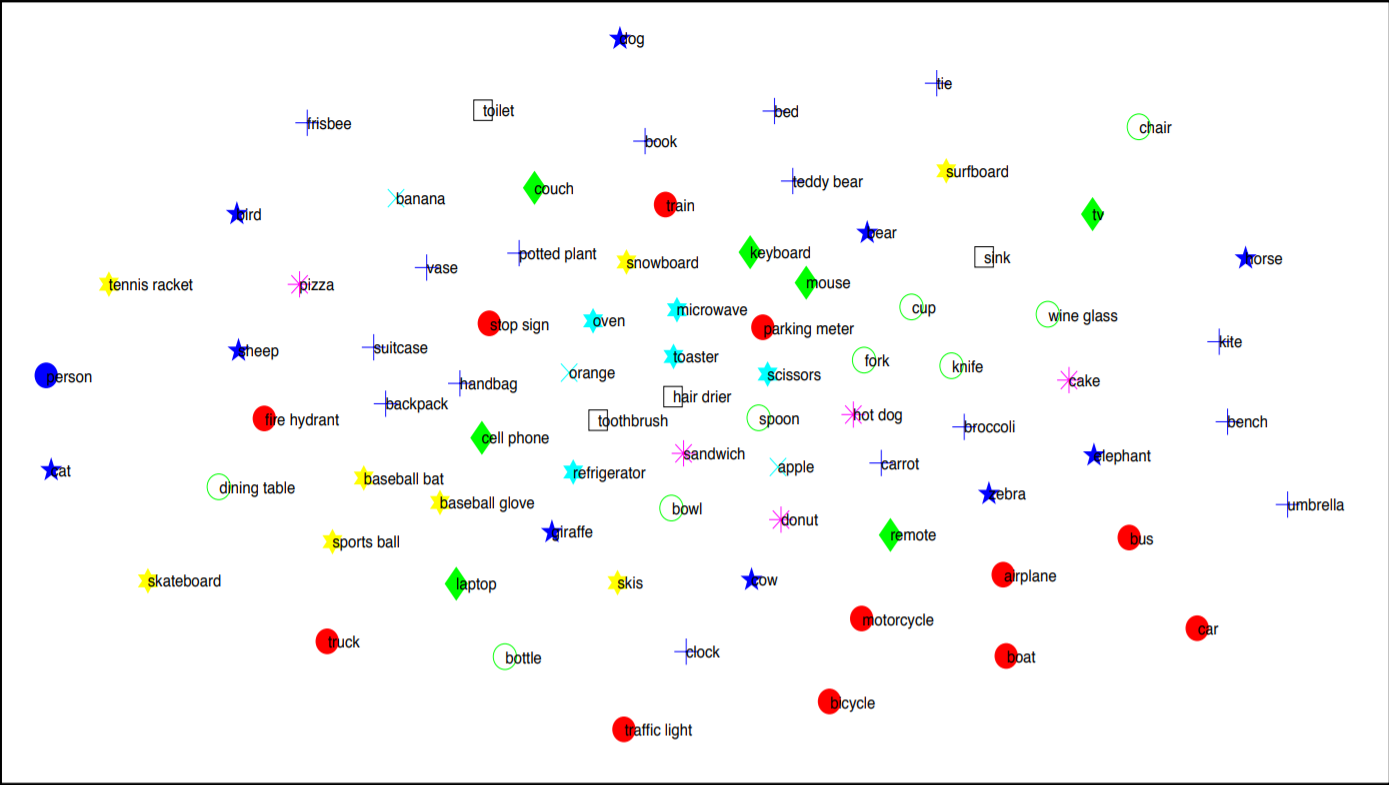
\includegraphics[scale=0.2]{/home/alex/python/Master_course/scientific_diary_2019-2020/slides/pics/Latent_multy_regular.png}
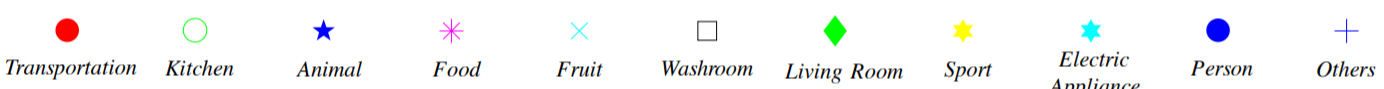
\includegraphics[scale=0.2]{/home/alex/python/Master_course/scientific_diary_2019-2020/slides/pics/Labels_multy.png}
\end{center}
\end{figure}

\end{frame}

\begin{frame}\frametitle{\footnotesize{Multi-Label Image Recognition with Graph Convolutional Networks\\
Zhao-Min Chen, Xiu-Shen Wei, Peng Wang, Yanwen Guo 2019 CVPR
}}
\begin{figure}[h]
\begin{center}
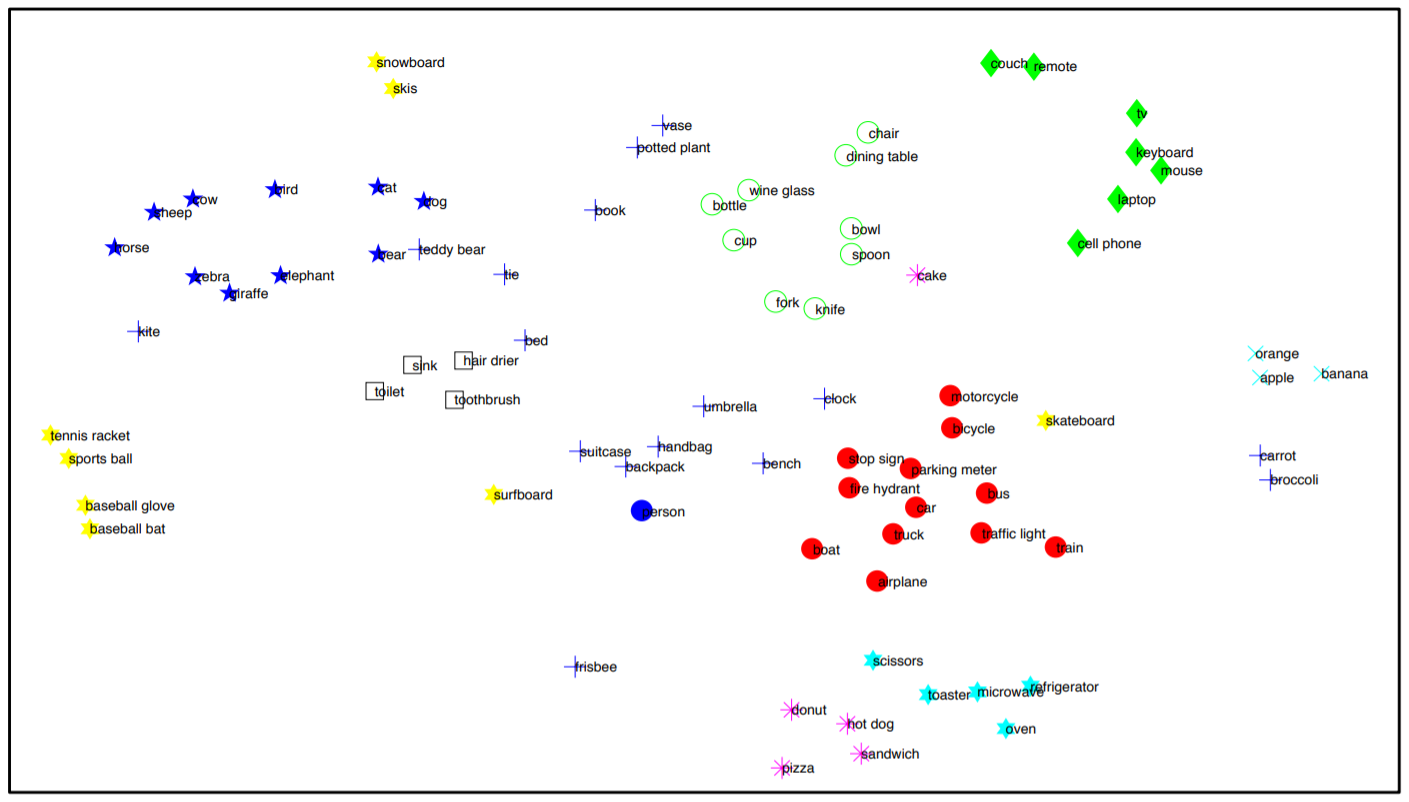
\includegraphics[scale=0.2]{/home/alex/python/Master_course/scientific_diary_2019-2020/slides/pics/Latent_multy.png}
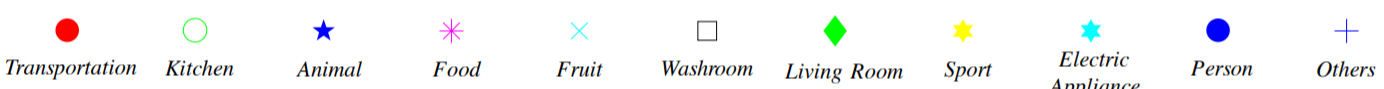
\includegraphics[scale=0.2]{/home/alex/python/Master_course/scientific_diary_2019-2020/slides/pics/Labels_multy.png}
\end{center}
\end{figure}

\end{frame}

\begin{frame}\frametitle{\footnotesize{Actional-Structural Graph Convolutional Networks for Skeleton-based Action Recognition 
Maosen Li , Siheng Chen, Xu Chen, Ya Zhang, Yanfeng Wang, and Qi Tian 2019 CVPR 
}}
\begin{table}[h!]
\begin{center}
\begin{tabular}{cc}
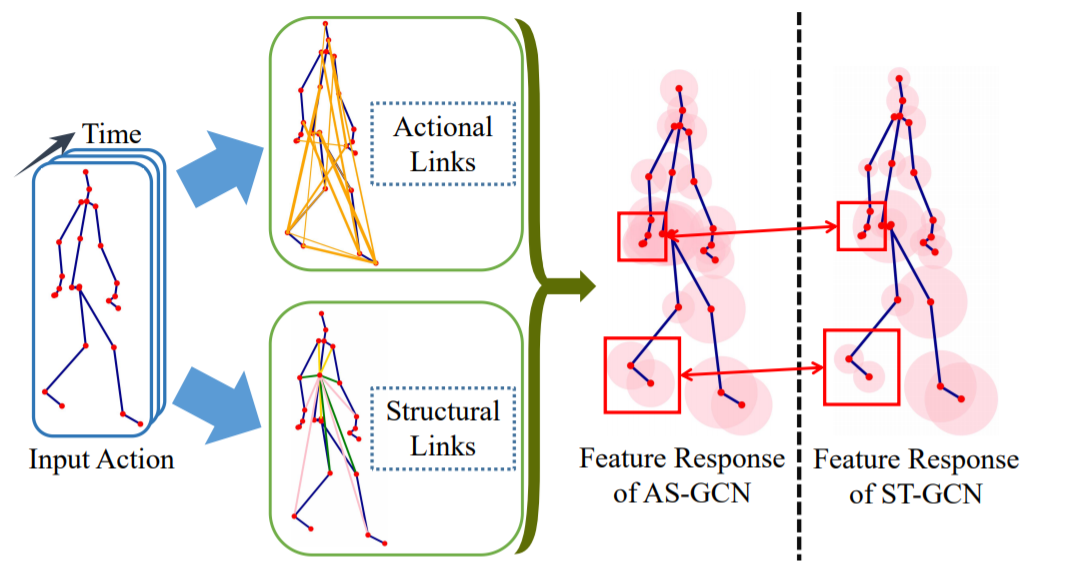
\includegraphics[scale=0.15]{/home/alex/python/Master_course/scientific_diary_2019-2020/slides/pics/Task_start_actlrec.png} &
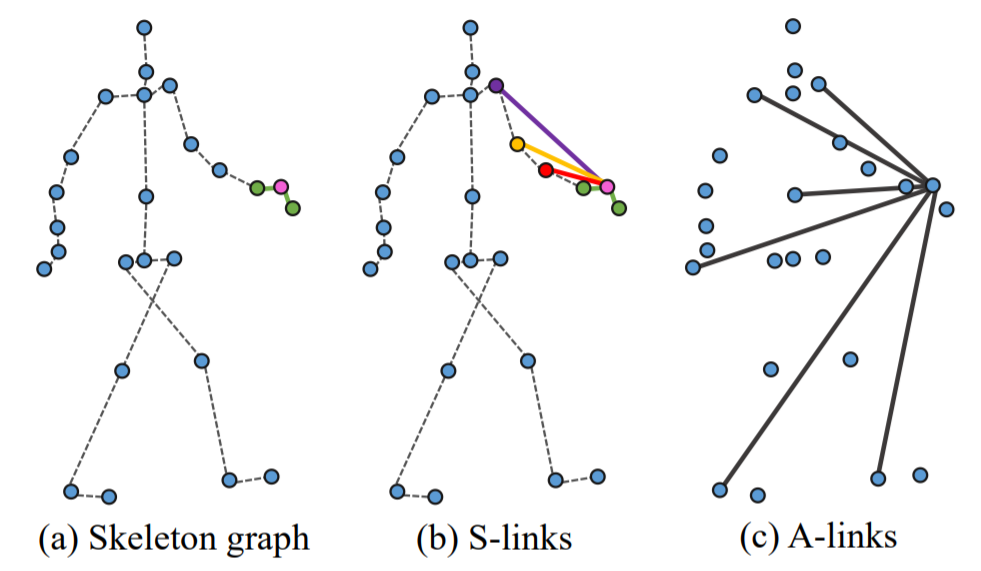
\includegraphics[scale=0.15]{/home/alex/python/Master_course/scientific_diary_2019-2020/slides/pics/Links_types_actrec.png}
\end{tabular}
\end{center}
\end{table}

\end{frame}

\begin{frame}\frametitle{\footnotesize{Actional-Structural Graph Convolutional Networks for Skeleton-based Action Recognition 
Maosen Li , Siheng Chen, Xu Chen, Ya Zhang, Yanfeng Wang, and Qi Tian 2019 CVPR 
}}
\begin{figure}[h]
\begin{center}
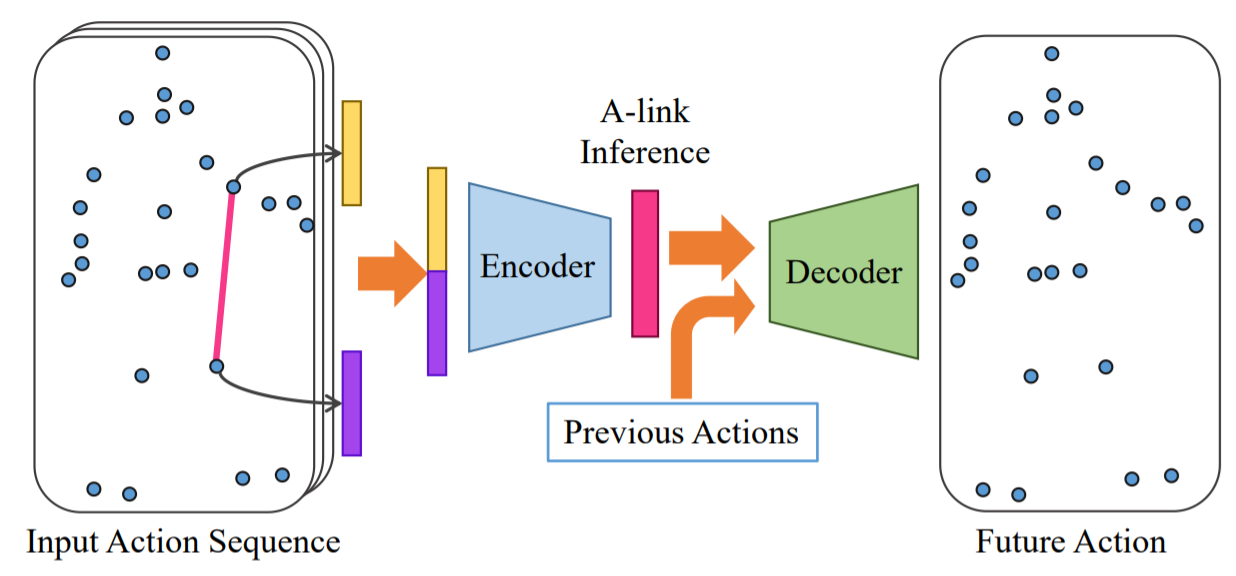
\includegraphics[scale=0.2]{/home/alex/python/Master_course/scientific_diary_2019-2020/slides/pics/AIM.png}
\end{center}
\end{figure}

\end{frame}	

\begin{frame}\frametitle{\footnotesize{Actional-Structural Graph Convolutional Networks for Skeleton-based Action Recognition 
Maosen Li , Siheng Chen, Xu Chen, Ya Zhang, Yanfeng Wang, and Qi Tian 2019 CVPR 
}}
\begin{block}{Encoder part}
link features:$ \mathbf{Q}^{k+1}_{ij} = f_e^k(f_v^k(p_i^k)\oplus f_v^k(p_j^k)),$\\
joint features:
$ p_i^{k+1}=\mathcal{F}(Q^{k+1})\oplus p_i^k$
$$\mathcal{A}_{i,j,:} = \mbox{softmax}\left( \frac{Q^K_{i,j}+r}{\tau} \right) \in \mathbb{R}^C$$
\end{block}

\begin{block}{Decoder part}
link features:$ \mathbf{Q}^{t}_{ij} = \sum \limits_{c=1}^C \mathcal{A}_{i,j,c} f_e^c(f_v^c(x_i^t)\oplus f_v^c(x_j^t)),$\\
joint features:
$ p_i^{t}=\mathcal{F}(Q^{t}_{i,:})\oplus x_i^t$\\
hidden state: $ S^{t+1}_i = GRU(S^t_i,p_i^t) $\\
expectation of position:$ \hat{\mu}^{t+1}_i = f_out(S^{t+1}_i)\in \mathbb{R}^3$
\end{block}

\end{frame}

\begin{frame}\frametitle{\footnotesize{Actional-Structural Graph Convolutional Networks for Skeleton-based Action Recognition 
Maosen Li , Siheng Chen, Xu Chen, Ya Zhang, Yanfeng Wang, and Qi Tian 2019 CVPR 
}}
\begin{block}{Loss}
$$ \mathcal{L}_{AIM}(\mathcal{A}) = -\sum_{i=1}^n\sum_{t=2}^T \frac{\Vert x_i^t - \hat{\mu}_i^t \Vert^2}{2\sigma^2} + \sum \limits_{c=1}^C \log \frac{\mathcal{A}_{:,:,c}}{\mathcal{A}^0_{:,:,c}} $$
\end{block}

\begin{block}{Prior}
$$\forall i,j,\; \mathcal{A}_{i,j,0} \sum \limits_{c=1}^C \mathcal{A}_{i,j,c} = 1,$$
$$ \mathcal{A}_{i,j,0}^0 = P_0,\; \mathcal{A}_{i,j,c}^0=P_0/C,\; \hat{A}_{act}^{(c)} = D_{act}^{(c)^-1} A_{act}^{(c)}$$

\end{block}

\begin{block}{AGC}
$$ X_act = AGC(X_{in}) = \sum_{c=1}^C \hat{A}_{act}^{(c)}X_{in}W_{act}^{(c)} \in \mathbb{R}^{n\times d_{out}}$$
\end{block}

\end{frame}

\begin{frame}\frametitle{\footnotesize{Actional-Structural Graph Convolutional Networks for Skeleton-based Action Recognition 
Maosen Li , Siheng Chen, Xu Chen, Ya Zhang, Yanfeng Wang, and Qi Tian 2019 CVPR 
}}

\begin{block}{Structural Convolution}
$$ \hat{A} = D^{-1}A $$
$$ X_struc = SGC(X_in) = \sum \limits_{l=1}^L \sum \limits_{p \in \mathcal{P}} M_{struc}^{(p,l)} \odot \hat{A}^{(p)l} X_{in}W_{struc}^{(p, l)} \in \mathbb{R}^{n \times d_{out}}$$
\end{block}

\end{frame}

\begin{frame}\frametitle{\footnotesize{Actional-Structural Graph Convolutional Networks for Skeleton-based Action Recognition 
Maosen Li , Siheng Chen, Xu Chen, Ya Zhang, Yanfeng Wang, and Qi Tian 2019 CVPR 
}}
\begin{figure}[h]
\begin{center}
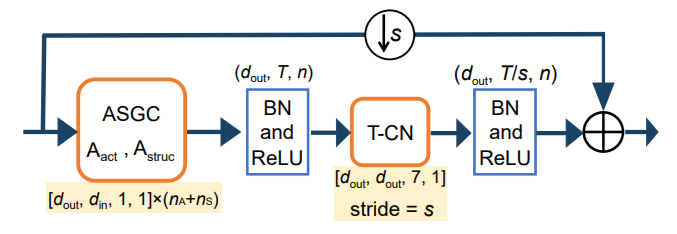
\includegraphics[scale=0.5]{/home/alex/python/Master_course/scientific_diary_2019-2020/slides/pics/AS-GCN.png}
\end{center}
\end{figure}

$$ \mathcal{L}_{recog} = -y^T \log(\hat{y}),\; \mathcal{L}_{predict} = \frac{1}{ndT'} \sum \limits_i^{nd}\sum \limits_{t=1}^{T'} \Vert \hat{\mathcal{X}}_{i,:,t} - \mathcal{X}_{i,:,t} \Vert^2_2$$ 

\end{frame}	

\begin{frame}\frametitle{\footnotesize{Actional-Structural Graph Convolutional Networks for Skeleton-based Action Recognition 
Maosen Li , Siheng Chen, Xu Chen, Ya Zhang, Yanfeng Wang, and Qi Tian 2019 CVPR 
}}

\begin{figure}[h]
\begin{center}
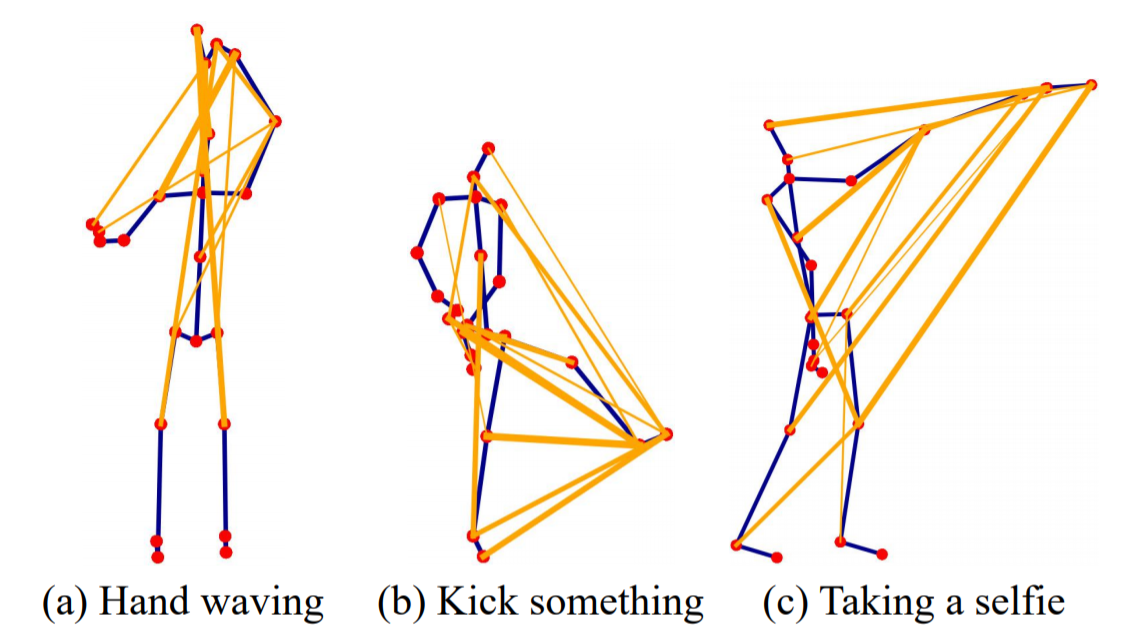
\includegraphics[scale=0.2]{/home/alex/python/Master_course/scientific_diary_2019-2020/slides/pics/act_link_vis.png}
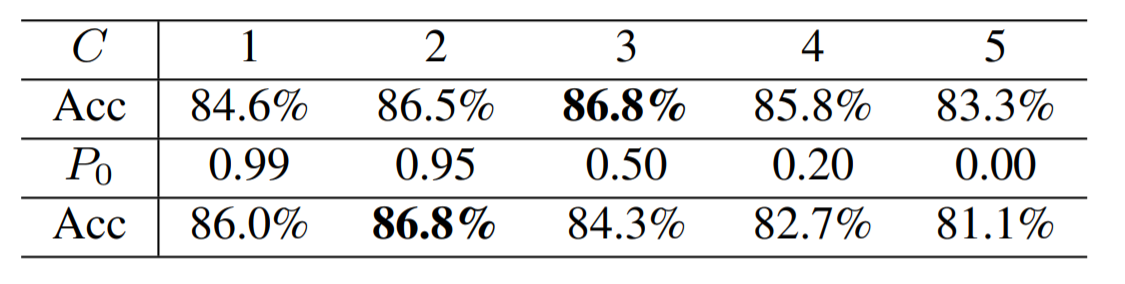
\includegraphics[scale=0.2]{/home/alex/python/Master_course/scientific_diary_2019-2020/slides/pics/alinks_perf_table.png}
\end{center}
\end{figure}

\end{frame}	

\begin{frame}\frametitle{\footnotesize{Actional-Structural Graph Convolutional Networks for Skeleton-based Action Recognition 
Maosen Li , Siheng Chen, Xu Chen, Ya Zhang, Yanfeng Wang, and Qi Tian 2019 CVPR 
}}

\begin{figure}[h]
\begin{center}
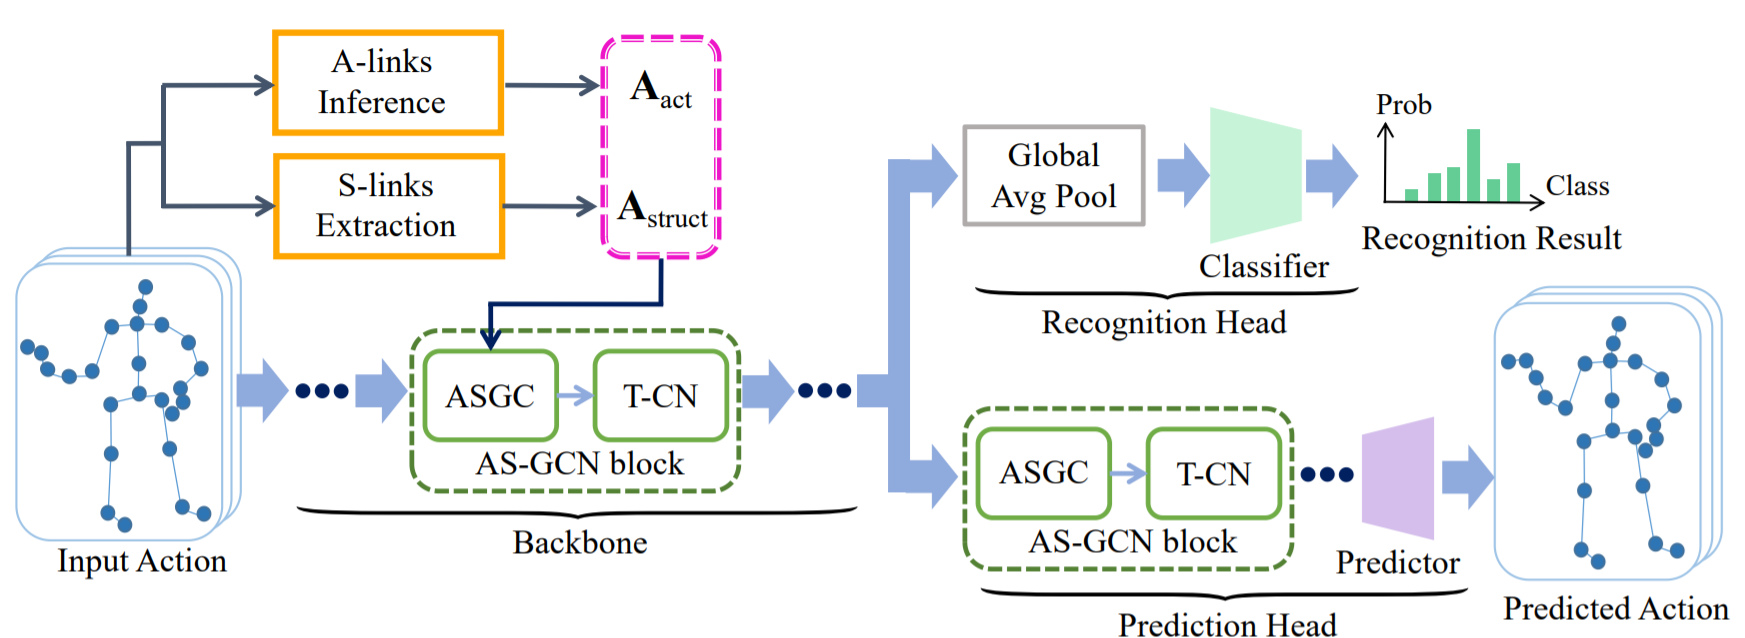
\includegraphics[scale=0.18]{/home/alex/python/Master_course/scientific_diary_2019-2020/slides/pics/ActionRec_scheme.png}
\end{center}
\end{figure}

\end{frame}	


\end{document}

